% Options for packages loaded elsewhere
\PassOptionsToPackage{unicode}{hyperref}
\PassOptionsToPackage{hyphens}{url}
\PassOptionsToPackage{dvipsnames,svgnames,x11names}{xcolor}
%
\documentclass[
  letterpaper,
]{article}

\usepackage{amsmath,amssymb}
\usepackage{lmodern}
\usepackage{iftex}
\ifPDFTeX
  \usepackage[T1]{fontenc}
  \usepackage[utf8]{inputenc}
  \usepackage{textcomp} % provide euro and other symbols
\else % if luatex or xetex
  \usepackage{unicode-math}
  \defaultfontfeatures{Scale=MatchLowercase}
  \defaultfontfeatures[\rmfamily]{Ligatures=TeX,Scale=1}
\fi
% Use upquote if available, for straight quotes in verbatim environments
\IfFileExists{upquote.sty}{\usepackage{upquote}}{}
\IfFileExists{microtype.sty}{% use microtype if available
  \usepackage[]{microtype}
  \UseMicrotypeSet[protrusion]{basicmath} % disable protrusion for tt fonts
}{}
\makeatletter
\@ifundefined{KOMAClassName}{% if non-KOMA class
  \IfFileExists{parskip.sty}{%
    \usepackage{parskip}
  }{% else
    \setlength{\parindent}{0pt}
    \setlength{\parskip}{6pt plus 2pt minus 1pt}}
}{% if KOMA class
  \KOMAoptions{parskip=half}}
\makeatother
\usepackage{xcolor}
\setlength{\emergencystretch}{3em} % prevent overfull lines
\setcounter{secnumdepth}{3}
% Make \paragraph and \subparagraph free-standing
\ifx\paragraph\undefined\else
  \let\oldparagraph\paragraph
  \renewcommand{\paragraph}[1]{\oldparagraph{#1}\mbox{}}
\fi
\ifx\subparagraph\undefined\else
  \let\oldsubparagraph\subparagraph
  \renewcommand{\subparagraph}[1]{\oldsubparagraph{#1}\mbox{}}
\fi


\providecommand{\tightlist}{%
  \setlength{\itemsep}{0pt}\setlength{\parskip}{0pt}}\usepackage{longtable,booktabs,array}
\usepackage{calc} % for calculating minipage widths
% Correct order of tables after \paragraph or \subparagraph
\usepackage{etoolbox}
\makeatletter
\patchcmd\longtable{\par}{\if@noskipsec\mbox{}\fi\par}{}{}
\makeatother
% Allow footnotes in longtable head/foot
\IfFileExists{footnotehyper.sty}{\usepackage{footnotehyper}}{\usepackage{footnote}}
\makesavenoteenv{longtable}
\usepackage{graphicx}
\makeatletter
\def\maxwidth{\ifdim\Gin@nat@width>\linewidth\linewidth\else\Gin@nat@width\fi}
\def\maxheight{\ifdim\Gin@nat@height>\textheight\textheight\else\Gin@nat@height\fi}
\makeatother
% Scale images if necessary, so that they will not overflow the page
% margins by default, and it is still possible to overwrite the defaults
% using explicit options in \includegraphics[width, height, ...]{}
\setkeys{Gin}{width=\maxwidth,height=\maxheight,keepaspectratio}
% Set default figure placement to htbp
\makeatletter
\def\fps@figure{htbp}
\makeatother

\makeatletter
\makeatother
\makeatletter
\makeatother
\makeatletter
\@ifpackageloaded{caption}{}{\usepackage{caption}}
\AtBeginDocument{%
\ifdefined\contentsname
  \renewcommand*\contentsname{Table of contents}
\else
  \newcommand\contentsname{Table of contents}
\fi
\ifdefined\listfigurename
  \renewcommand*\listfigurename{List of Figures}
\else
  \newcommand\listfigurename{List of Figures}
\fi
\ifdefined\listtablename
  \renewcommand*\listtablename{List of Tables}
\else
  \newcommand\listtablename{List of Tables}
\fi
\ifdefined\figurename
  \renewcommand*\figurename{Figure}
\else
  \newcommand\figurename{Figure}
\fi
\ifdefined\tablename
  \renewcommand*\tablename{Table}
\else
  \newcommand\tablename{Table}
\fi
}
\@ifpackageloaded{float}{}{\usepackage{float}}
\floatstyle{ruled}
\@ifundefined{c@chapter}{\newfloat{codelisting}{h}{lop}}{\newfloat{codelisting}{h}{lop}[chapter]}
\floatname{codelisting}{Listing}
\newcommand*\listoflistings{\listof{codelisting}{List of Listings}}
\makeatother
\makeatletter
\@ifpackageloaded{caption}{}{\usepackage{caption}}
\@ifpackageloaded{subcaption}{}{\usepackage{subcaption}}
\makeatother
\makeatletter
\@ifpackageloaded{tcolorbox}{}{\usepackage[many]{tcolorbox}}
\makeatother
\makeatletter
\@ifundefined{shadecolor}{\definecolor{shadecolor}{rgb}{.97, .97, .97}}
\makeatother
\makeatletter
\makeatother
\ifLuaTeX
  \usepackage{selnolig}  % disable illegal ligatures
\fi
\usepackage[]{biblatex}
\addbibresource{../../../../references.bib}
\IfFileExists{bookmark.sty}{\usepackage{bookmark}}{\usepackage{hyperref}}
\IfFileExists{xurl.sty}{\usepackage{xurl}}{} % add URL line breaks if available
\urlstyle{same} % disable monospaced font for URLs
\hypersetup{
  pdftitle={Cómo usar APK en Windows 11 una guía paso a paso},
  pdfauthor={Edison Achalma Mendoza},
  colorlinks=true,
  linkcolor={blue},
  filecolor={Maroon},
  citecolor={Blue},
  urlcolor={Blue},
  pdfcreator={LaTeX via pandoc}}

\title{Cómo usar APK en Windows 11 una guía paso a paso}
\usepackage{etoolbox}
\makeatletter
\providecommand{\subtitle}[1]{% add subtitle to \maketitle
  \apptocmd{\@title}{\par {\large #1 \par}}{}{}
}
\makeatother
\subtitle{Aprende a instalar y ejecutar aplicaciones de Android en tu PC
con Windows 11}
\author{Edison Achalma Mendoza}
\date{9/27/22}

\begin{document}
\maketitle
\ifdefined\Shaded\renewenvironment{Shaded}{\begin{tcolorbox}[frame hidden, borderline west={3pt}{0pt}{shadecolor}, enhanced, boxrule=0pt, breakable, interior hidden, sharp corners]}{\end{tcolorbox}}\fi

\renewcommand*\contentsname{Contenidos}
{
\hypersetup{linkcolor=}
\setcounter{tocdepth}{3}
\tableofcontents
}
\hypertarget{windows-11-cuxf3mo-descargar-apk-usando-el-subsistema-de-windows-para-android-y-adb}{%
\section{Windows 11: Cómo descargar APK usando el subsistema de Windows
para Android y
ADB}\label{windows-11-cuxf3mo-descargar-apk-usando-el-subsistema-de-windows-para-android-y-adb}}

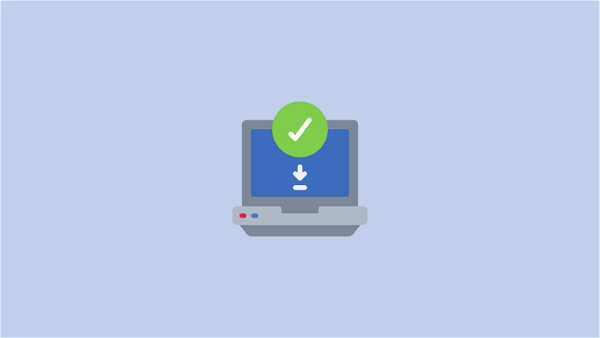
\includegraphics{https://cdn.nerdschalk.com/wp-content/uploads/2021/10/install-logo-759x427.png?width=600}

Aquí se explica cómo descargar un archivo APK para instalar la
aplicación de Android en su PC con Windows 11 usando el Subsistema de
Windows para Android.~Puede instalar Windows Subsystem para Android
manualmente en su PC con Windows 11 usando su archivo Msixbundle de
nuestra~\href{https://nerdschalk.com/android-apps-on-windows-11-dev-channel-how-to-install-windows-subsystem-for-android-manually-with-msixbundle/}{guía
aquí}~.

\href{https://nerdschalk.com/windows-11-how-to-sideload-apk-using-windows-subsystem-for-android-and-adb/\#}{Mostrar}~\textbf{CONTENIDO}~\href{https://nerdschalk.com/windows-11-how-to-sideload-apk-using-windows-subsystem-for-android-and-adb/\#}{}

\hypertarget{paso-1-habilite-el-modo-de-desarrollador-en-el-subsistema-de-windows}{%
\subsection{Paso 1: habilite el modo de desarrollador en el subsistema
de
Windows}\label{paso-1-habilite-el-modo-de-desarrollador-en-el-subsistema-de-windows}}

Instale~\href{https://nerdschalk.com/android-apps-on-windows-11-dev-channel-how-to-install-windows-subsystem-for-android-manually-with-msixbundle/}{el
Subsistema de Windows para Android}~primero.~Cuando haya terminado, abra
la aplicación `Subsistema de Windows para Android' en su PC.~Para esto,
presione la tecla de Windows y busque Subsistema de Windows para
Android.

\includegraphics{https://cdn.nerdschalk.com/wp-content/uploads/2021/10/get-android-apps-on-windows-11-dev-channel-09.png?width=800}

Haga clic en Subsistema de Windows para Android.~O haga clic en Abrir.

\includegraphics{https://cdn.nerdschalk.com/wp-content/uploads/2021/10/get-android-apps-on-windows-11-dev-channel-08.png?width=800}

En el Subsistema de Windows para Android, active el modo Desarrollador.

\includegraphics{https://cdn.nerdschalk.com/wp-content/uploads/2021/10/get-android-apps-on-windows-11-dev-channel-10-2.png?width=800}

\hypertarget{paso-2-instale-las-herramientas-de-la-plataforma-sdk}{%
\subsection{Paso 2: Instale las herramientas de la plataforma
SDK}\label{paso-2-instale-las-herramientas-de-la-plataforma-sdk}}

Visite la página de herramientas de la plataforma SDK de
Google~\href{https://developer.android.com/studio/releases/platform-tools.html}{aquí}~.

Haga clic en Descargar SDK Platform-Tools para Windows.

\includegraphics{https://cdn.nerdschalk.com/wp-content/uploads/2021/10/get-android-apps-on-windows-11-dev-channel-11.png?width=800}

Desplácese hacia abajo hasta el final y seleccione la casilla de
verificación para aceptar los términos y condiciones.~Luego haga clic en
el botón verde para descargar las herramientas de la plataforma.

\includegraphics{https://cdn.nerdschalk.com/wp-content/uploads/2021/10/get-android-apps-on-windows-11-dev-channel-12.png?width=700}

Se descargará en su PC un archivo zip llamado
platform-tools\_r31.0.3-windows (la versión puede cambiar).

\includegraphics{https://cdn.nerdschalk.com/wp-content/uploads/2021/10/get-android-apps-on-windows-11-dev-channel-13.png?width=700}

Para su comodidad, cree una nueva carpeta separada llamada carpeta para
aplicaciones en el Explorador de Windows.~Ahora, transfiera el archivo
de herramientas de la plataforma a esta carpeta.

Haga clic con el botón derecho en el archivo de herramientas de la
plataforma y seleccione Extraer todo.

\includegraphics{https://cdn.nerdschalk.com/wp-content/uploads/2021/10/get-android-apps-on-windows-11-dev-channel-14.png?width=500}

Haga clic en Extraer.

\includegraphics{https://cdn.nerdschalk.com/wp-content/uploads/2021/10/get-android-apps-on-windows-11-dev-channel-15-2.png?width=700}

El archivo será extraído.~Abra la carpeta llamada herramientas de la
plataforma.

\includegraphics{https://cdn.nerdschalk.com/wp-content/uploads/2021/10/get-android-apps-on-windows-11-dev-channel-16.png?width=500}

Tendrá adb.exe y algunos otros archivos aquí.

\textbf{Relacionado:}~\href{https://nerdschalk.com/how-to-restart-windows-explorer-on-windows-11-and-what-happens-when-you-do-it/}{Cómo
reiniciar el Explorador de Windows en Windows 11 y qué sucede cuando lo
hace}

\hypertarget{paso-3-instale-la-aplicaciuxf3n-de-android}{%
\subsection{Paso 3: Instale la aplicación de
Android}\label{paso-3-instale-la-aplicaciuxf3n-de-android}}

Haga doble clic en la carpeta de herramientas de la plataforma para
abrirla.

Aquí, haga clic en la barra de direcciones y escriba~\textbf{cmd,}~y
luego presione la tecla Intro.

\includegraphics{https://cdn.nerdschalk.com/wp-content/uploads/2021/10/get-android-apps-on-windows-11-dev-channel-20.png?width=500}

Se abrirá una ventana de comando con su ubicación establecida en la
carpeta de herramientas de la plataforma.~Esto es importante.

\includegraphics{https://cdn.nerdschalk.com/wp-content/uploads/2021/10/get-android-apps-on-windows-11-dev-channel-21.png?width=800}

Ahora, tenemos la ventana del símbolo del sistema en la carpeta donde
tenemos el archivo adb.exe.~Es decir, nuestra carpeta de herramientas de
plataforma.

\includegraphics{https://cdn.nerdschalk.com/wp-content/uploads/2021/10/get-android-apps-on-windows-11-dev-channel-17.png?width=700}

Ahora, descargue el archivo APK de la aplicación de Android que desea
instalar.~Por ejemplo, si desea instalar Snapchat,
busque~\textbf{Snapchat APK}~en Google y descargue su archivo APK desde
cualquier sitio web confiable en el que confíe.~Luego, cambie el nombre
del archivo a algo más simple como snapchat.apk.~Ahora, transfiera
snapchat.apk a la carpeta de herramientas de la plataforma.

\includegraphics{https://cdn.nerdschalk.com/wp-content/uploads/2021/10/get-android-apps-on-windows-11-dev-channel-18.png?width=700}

Ahora podemos instalar la aplicación Snapchat para Android usando
snapchat.apk y adb en su PC.

Abra el Subsistema de Windows para Android y busque la IP donde se puede
conectar con ADB en la opción de modo Desarrollador.

\includegraphics{https://cdn.nerdschalk.com/wp-content/uploads/2021/10/get-android-apps-on-windows-11-dev-channel-19.png?width=800}

En la ventana del símbolo del sistema, escriba el siguiente comando y
presione Entrar:

adb.exe connect (dirección IP-aquí)

Ejemplo: adb.exe conectar 127.0.0.1:12345

\includegraphics{https://cdn.nerdschalk.com/wp-content/uploads/2021/10/get-android-apps-on-windows-11-dev-channel-22.png?width=800}

Ahora, escriba el comando de instalación que se proporciona a
continuación y luego presione Enter:

adb.exe install (apk-file-name-here.apk)

Ejemplo: adb.exe instalar Snapchat.apk

\includegraphics{https://cdn.nerdschalk.com/wp-content/uploads/2021/10/get-android-apps-on-windows-11-dev-channel-23.png?width=800}

La aplicación de Android ahora se instalará en su PC usando ADB y el
archivo APK que proporcionó.

\includegraphics{https://cdn.nerdschalk.com/wp-content/uploads/2021/10/get-android-apps-on-windows-11-dev-channel-24.png?width=800}

Cuando haya terminado, verá el mensaje de Éxito.

\includegraphics{https://cdn.nerdschalk.com/wp-content/uploads/2021/10/get-android-apps-on-windows-11-dev-channel-25.png?width=800}

Puede cerrar la ventana CMD ahora.

Ahora puede abrir la aplicación de Android en su PC.

Presione la tecla de Windows y luego escriba el nombre de su
aplicación.~En nuestro caso, es Snapchat.

\includegraphics{https://cdn.nerdschalk.com/wp-content/uploads/2021/10/get-android-apps-on-windows-11-dev-channel-27.png?width=800}

Así es como se ve Snapchat en Windows 11.

\includegraphics{https://cdn.nerdschalk.com/wp-content/uploads/2021/10/get-android-apps-on-windows-11-dev-channel-26.jpg?width=800}

Eso es todo.

\hypertarget{cargar-apk-automuxe1ticamente-con-un-doble-clic}{%
\subsection{Cargar APK automáticamente con un doble
clic}\label{cargar-apk-automuxe1ticamente-con-un-doble-clic}}

Sabemos que usar un comando adb no es la forma más fácil de instalar una
aplicación de Android en su PC.~Afortunadamente, ahora puede hacer doble
clic en un archivo APK para instalarlo.~Consulta el siguiente enlace
para saber cómo configurarlo.

\textbf{Leer:}~\href{https://nerdschalk.com/how-to-sideload-apk-on-windows-11-automatically-with-a-double-click/}{Cómo
descargar APK en Windows 11 automáticamente con un doble clic}

Háganos saber cuál es su método favorito para cargar archivos APK en la
PC.

\textbf{RELACIONADO}

\begin{itemize}
\tightlist
\item
  \href{https://nerdschalk.com/how-to-disable-vbs-on-windows-11-and-does-it-help/}{¿Cómo
  deshabilitar VBS en Windows 11 y ayuda?}
\item
  \href{https://nerdschalk.com/first-10-things-to-do-on-windows-11/}{Las
  10 primeras cosas que hacer en Windows 11}
\item
  \href{https://nerdschalk.com/windows-11-how-to-create-live-tiles-and-widgets/}{Windows
  11: Cómo crear mosaicos y widgets en vivo usted mismo}
\item
  \href{https://nerdschalk.com/how-to-extend-volume-windows-11-or-windows-10/}{Cómo
  extender el volumen de Windows 11 o Windows 10}
\item
  \href{https://nerdschalk.com/how-to-facetime-windows-users/}{Cómo usar
  Facetime en
  Windows}~~\textbar~\href{https://nerdschalk.com/how-to-facetime-android-users/}{Androide}
\item
  \href{https://nerdschalk.com/how-to-calibrate-monitor-on-windows-11-pc/}{Cómo
  calibrar el monitor en una PC con Windows 11}
\item
  \href{https://nerdschalk.com/how-to-run-old-games-on-windows-11/}{Cómo
  ejecutar juegos antiguos en Windows 11}
\end{itemize}

\href{https://nerdschalk.com/tag/how-to/}{cómo}\href{https://nerdschalk.com/tag/windows-11/}{ventanas
11}

{[}

\includegraphics{https://secure.gravatar.com/avatar/8ddaa30f5018c02bbfc30545a9a2b72a?s=96\&d=retro\&r=g.pdf}

{]}(https://nerdschalk.com/author/ka1385/)

{[}publicado por

kapil malani

{]}(https://nerdschalk.com/author/ka1385/)

Aficionado acérrimo del Liverpool FC, Kapil es un gran admirador de
Batman, Android y Street Cricket.~En ese orden, probablemente.~Correo
electrónico:~kapil@theandroidsoul.com


\printbibliography


\end{document}
